\documentclass[14pt]{extarticle}

\usepackage[T1]{fontenc}
\usepackage[utf8]{inputenc}
\usepackage[russian]{babel}

% page margin
\usepackage[top=2cm, bottom=2cm, left=2cm, right=2cm]{geometry}

% AMS packages
\usepackage{amsmath}
\usepackage{amssymb}
\usepackage{amsfonts}
\usepackage{amsthm}

\usepackage{float}
\usepackage{graphicx}
\usepackage{tabularx}
\usepackage{multirow}

\newcommand{\lb}{\left(}
\newcommand{\rb}{\right)}

\makeatletter
\setlength{\@fptop}{0pt}
\makeatother

\begin{document}

\section*{Задача 3.}
В рамках приближения Борна свободная энергия гидратации электрона $\Delta G_s$ связана с термодинамическим радиусом гидратированного электрона $r_i$ следующим соотношением:
\begin{gather}
	- \Delta G_s = N_A \frac{z_i^2 e_0^2}{8 \pi \varepsilon_0 r_i} \lb 1 - \frac{1}{\varepsilon} \rb \quad \implies \quad r_i = - \frac{1}{\Delta G_s} N_A \frac{z_i^2 e_0^2}{8 \pi \varepsilon_0} \lb 1 - \frac{1}{\varepsilon} \rb \notag
\end{gather}

Данные по температурной зависимости диэлектрической постоянной были взяты из [1]. По экспериментальным точкам был положен кубический сплайн, чтобы получить интерполированные значение при $T = 298$K и $360$K (Рис. \ref{spline}).

\begin{figure}[H]
	\centering
	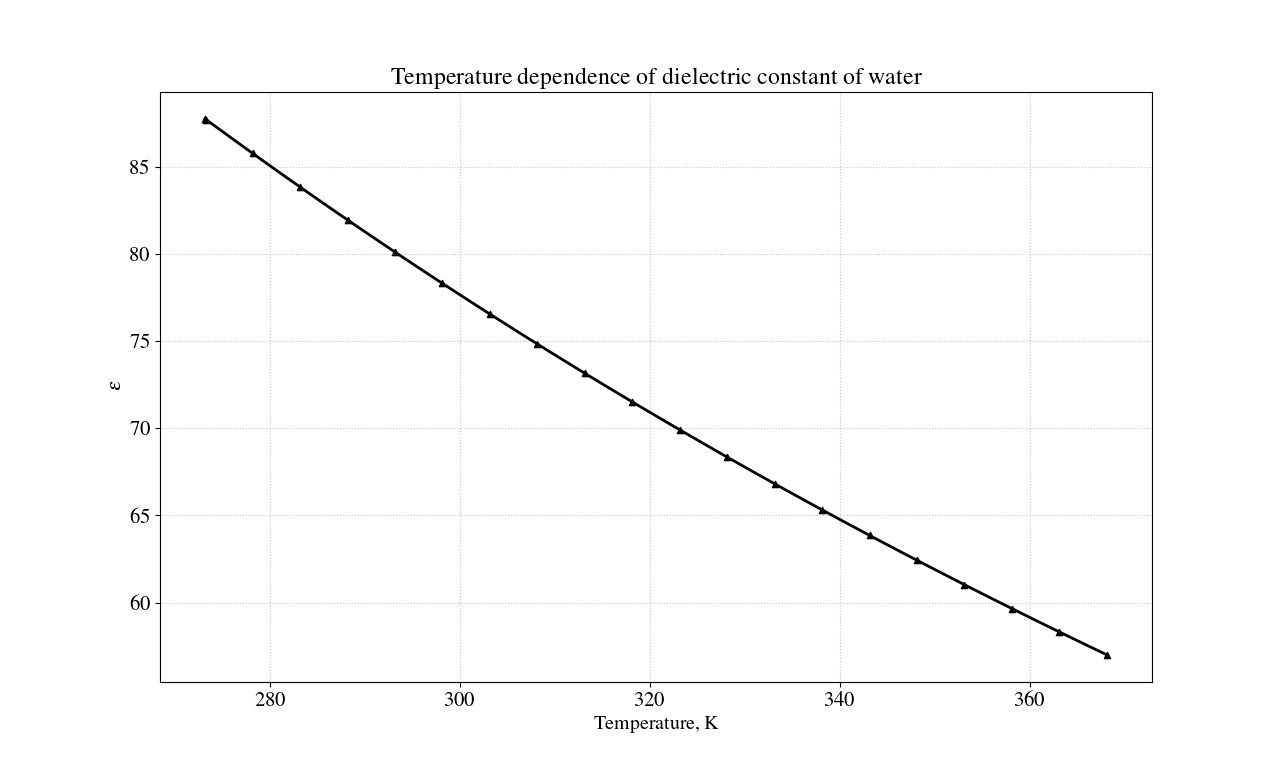
\includegraphics[width = 0.8\linewidth]{../pictures/dielec.png}
	\caption{Температурная зависимость диэлектрической постоянной [1]}
	\label{spline}
\end{figure}

\vspace*{-1cm}

\begin{gather}
	\varepsilon (298 K) =  78.357 \notag \\
	\varepsilon (360 K) =  59.159 \notag
\end{gather}

Термодинамический радиус гидратированного электрона в рамках борновского приближения при $T = 298$ K:
\begin{gather}
	r_i = 4.37 \textup{\AA} \notag
\end{gather}

Радиус получается завышенным; в первой лекции фигурировало значение полости $R_0 = 1.4-1.5$ \AA.

\begin{table}[H]
	\centering
	\begin{tabular}{|c|c|c|}
		\hline
		Ион & $r_i$, \AA & $-\Delta G_s$, кДж/моль \\ \hline 
		F$^{-}$ & 1.60 & 429 \\
		Cl$^{-}$ & 2.26 & 304 \\
		Br$^{-}$ & 2.47 & 278 \\
		I$^{-}$ & 2.82 & 243 \\ \hline
	\end{tabular}
	\caption{Значения свободной энергии гидратации [2] и борновских радиусов галоид-анионов}
\end{table}

Борновский радиус гидратированного электрона превышает борновские радиусы всех галоид-анионов. \par 
Согласно модели полости (digger mechanism), в растворителе образуется полость, в которой локализуется электрон. Внутри этой полости энергия электрона ниже, чем вне ее. Снижение энергии электрона вызвано тем, что он создает вокруг себя электрическое поле, ориентирующее полярные молекулы растворителя. Таким образом, в результате такой поляризации, вокруг электрона создается своего рода "ловушка". Однако потенциальный барьер такой ловушки не является высоким, электрон легко перескакивает между полостями. Размер полости не является определенной величиной, а имеет распределенный характер. Термодинамически оцененный гидратированный размер электрона является средним значением размеров полостей. В условиях определения кинетического радиуса ориентационные взаимодействия, вызванные полем электрона, в большей степени компенсируются общим движением средыпо сравнению со стационарными условиями. Меньший размер полостей приводит к меньшему кинетическому размеру.  

Предполагая, что борновский радиус $r_i$ не зависит от температуры, получим оценку $\Delta G_s(360K)$:
\begin{gather}
		\Delta G_s = - N_A \frac{z_i e_0^2}{8 \pi \varepsilon_0 r_i} \lb 1 - \frac{1}{\varepsilon} \rb = -156.34 \, \textup{кДж/моль} \notag
\end{gather}

Рассчитанные значения $\Delta G_s$ в борновском приближении обычно превышают экспериментальные значения.

\subsection*{Список литературы}

\begin{enumerate}
	\item Malmberg, C.G. and Maryott, A.A., 1956. Dielectric Constant of Water from 0 to 100 C. Journal of research of the National Bureau of Standards, 56(1), pp.1-8.
	\item Fawcett, W.R., 1999. Thermodynamic parameters for the solvation of monatomic ions in water. The Journal of Physical Chemistry B, 103(50), pp.11181-11185. 
\end{enumerate}


\end{document}
